% =========================================================================
% Real-time interactive inference for world models.
% arXiv preprint. Measured results and planned follow-up work are
% distinguished explicitly.
% Build: pdflatex master.tex && pdflatex master.tex
% Figures: python make_paper_figures.py (result plots); Figure 1 is TikZ.
% =========================================================================
\documentclass[11pt]{article}
\usepackage[margin=1in]{geometry}
\usepackage{amsmath,amssymb}
\usepackage{booktabs}
\usepackage{array,tabularx}
\usepackage{graphicx}
\usepackage{tikz}
\usetikzlibrary{decorations.pathreplacing,arrows.meta,positioning}
\usepackage{float}
\usepackage[colorlinks=true,linkcolor=blue,citecolor=blue,urlcolor=blue]{hyperref}
\usepackage{xcolor}
\newcommand{\planned}[1]{\emph{Planned follow-up:} #1}
\newcommand{\caol}{CAOL}
\newcolumntype{L}[1]{>{\raggedright\arraybackslash}p{#1}}
\newcolumntype{C}[1]{>{\centering\arraybackslash}p{#1}}
\newcolumntype{Y}{>{\raggedright\arraybackslash}X}
\definecolor{figgreen}{HTML}{2d6a4f}
\definecolor{figorange}{HTML}{ca6702}
\definecolor{figred}{HTML}{ae2012}
\definecolor{figgray}{HTML}{6c757d}
\newcommand{\ExpectedPairs}{24}
\newcommand{\ValidPairs}{24}
\newcommand{\ShortAdmissionFrames}{12}
\newcommand{\ShortAnyDetection}{100\%}
\newcommand{\ShortBothDetection}{100\%}
\newcommand{\ShortOnsetLag}{9.0 [9.0, 9.0]}
\newcommand{\ShortFPS}{0.834309 [0.831234, 0.837557]}
\newcommand{\ShortEffectPeak}{0.0172288 [0.0170293, 0.0174545]}
\newcommand{\ShortFrameReadyMs}{21476.2}
\newcommand{\ShortFrameReadySDMs}{29.2}
\newcommand{\LongAdmissionFrames}{24}
\newcommand{\LongAnyDetection}{100\%}
\newcommand{\LongBothDetection}{100\%}
\newcommand{\LongOnsetLag}{21.0 [21.0, 21.0]}
\newcommand{\LongFPS}{0.835026 [0.831762, 0.838335]}
\newcommand{\LongEffectPeak}{0.0171567 [0.0168052, 0.0174573]}
\newcommand{\LongFrameReadyMs}{32930.3}
\newcommand{\LongFrameReadySDMs}{958.3}
\newcommand{\RelativeThroughputDifference}{0.085889\%}
\newcommand{\IncrementalRunCount}{4}
\newcommand{\IncrementalMaxError}{0}
\newcommand{\IncrementalDroppedFrames}{0}
\newcommand{\RFProbeCount}{24}
\newcommand{\DirectionalInterventions}{24}
\newcommand{\DirectionalCausalDivergence}{100\%}
\newcommand{\DirectionalObedience}{failed}
\newcommand{\VPTEpisodes}{597}
\newcommand{\VPTTestEpisodes}{85}
\newcommand{\VPTEligibleBlocks}{28,310}
\newcommand{\VPTChangeBlocks}{21,397}
\newcommand{\IntentOverallHit}{59.1381\%}
\newcommand{\IntentOverallCI}{[56.7646,61.4038]\%}
\newcommand{\IntentChangesHit}{47.3197\%}
\newcommand{\IntentChangesCI}{[44.4826,50.1101]\%}
\newcommand{\StrictOverallHit}{9.6044\%}
\newcommand{\StrictOverallCI}{[7.5837,11.7939]\%}
\newcommand{\StrictChangesHit}{2.0984\%}
\newcommand{\StrictChangesCI}{[1.7437,2.4700]\%}
\newcommand{\GammaCandidateRange}{4.70--4.72\,s}
\newcommand{\GammaChargedWork}{89.764\,s}
\newcommand{\GammaBranchStateGB}{4.9656\,GB}
\newcommand{\ProjectedReadiness}{0\%}
\newcommand{\ProposalCheckpointCount}{44}
\newcommand{\ProposalMaxError}{0}
\newcommand{\PreRollProposalMedianMs}{500.74}
\newcommand{\PreRollProposalTailMs}{506.53}
\newcommand{\PreRollCommitSaveTailMs}{484.20}
\newcommand{\PreRollHostSaveTailMs}{541.41}
\newcommand{\PreRollEligibleDecisions}{582}
\newcommand{\PreRollEligibleFraction}{2.06\%}
\newcommand{\FirstRollProposalTailMs}{1752.99}
\newcommand{\SteadyRollProposalTailMs}{1754.88}
\newcommand{\ExactConfidenceCoverage}{2.41\%}
\newcommand{\ExactConfidencePrecision}{42.86\%}
\newcommand{\ExactConfidenceWorkDeltaMs}{3440.75}
\newcommand{\IntentProposalTailMs}{1596.02}
\newcommand{\IntentLatentMSE}{1.45747}
\newcommand{\IntentContinuationMSE}{2.69636}
\newcommand{\IntentPSNR}{7.839/8.215}
\newcommand{\IntentSSIM}{0.683/0.759}
\newcommand{\CowForkMedianUs}{5.01}
\newcommand{\CowCopyMedianMs}{3.29}


\title{Control-Aligned Onset Latency and\\
Copy-on-Write Speculative Branching for Streaming World Models}
\author{%
Arunkumar Eli$^{1}$ \qquad Vasu Sharma$^{2}$\\[0.4em]
\small $^{1}$Independent Research \qquad $^{2}$Pocket FM
}
\date{\textsc{A Preprint}}

\begin{document}
\maketitle
\vspace{-1.6em}

\begin{abstract}
\footnotesize
Interactive world models are commonly evaluated by frame rate, but a model can emit frames continuously while acting on stale controls. We introduce \emph{control-aligned onset latency} (\caol{}) and use matched unchanged-action rollouts to identify divergence attributable to the changed action under deterministic matched conditions. All \ValidPairs{}/\ExpectedPairs{} planned STOP pairs are valid: both/any-view detection is $100\%$, paired flow-divergence onset is $9$ versus $21$ frames, and effective throughput is $0.834$ versus $0.835$ FPS. Exact cached incremental decoding reaches host readiness in $21.48$ versus $32.93$\,s ($n=2$ per policy) with exact raw-uint8 output and no dropped frames; physical presentation is not measured. Forward-to-back and true-yaw interventions also produce paired divergence in both scenes, but the signed-direction audit fails, so directional obedience is not supported. For speculative branching, all \ProposalCheckpointCount{} completed checks of an exact uncommitted one-plus-three transaction match their references with zero error; the requested eight-block continuation could not run because it exceeds the tokenizer horizon. An initial-block proposal passes the 750\,ms readiness criterion, but later unsaturated readiness was not measured; proposals at the first and steady rolling boundaries exceed 1.75\,s, and exact selection increases proposal-inclusive compute. No general profitable speedup is established, and paged copy-on-write remains a separate allocator primitive.
\end{abstract}

\vspace{-0.35em}
\begin{center}
\small\textbf{Keywords:} streaming world models $\cdot$ control-aligned onset latency $\cdot$ interactive inference $\cdot$ diffusion serving\\[0.3em]
\small\textbf{Code and data:} \url{https://github.com/arun-elr/caol-streaming-world-models}
\end{center}
\vspace{-0.75em}

\begin{figure}[H]
\centering
\resizebox{0.78\textwidth}{!}{%
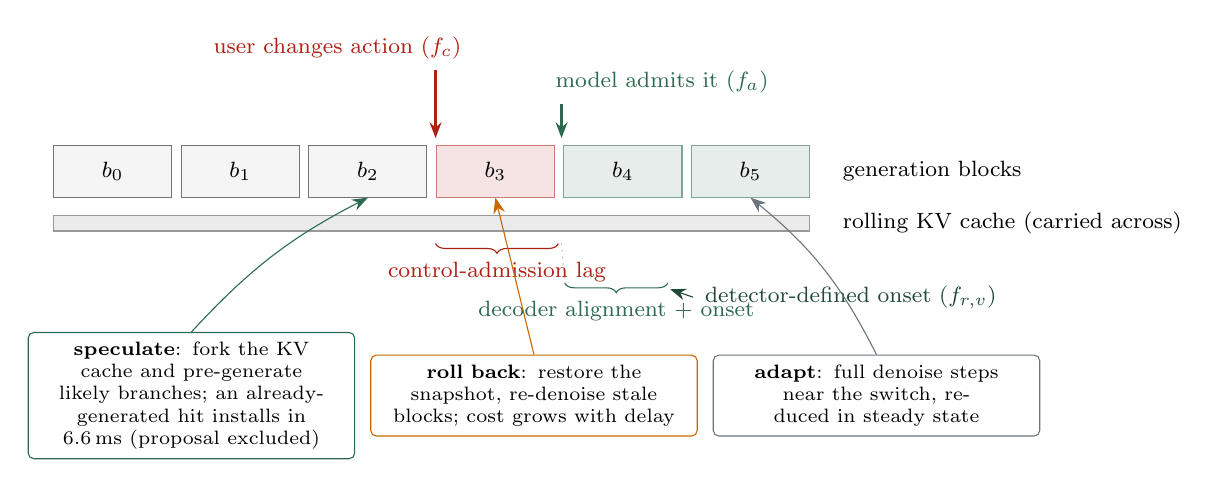
\begin{tikzpicture}[
  block/.style={draw=black!55, fill=black!4, minimum width=1.5cm, minimum height=0.66cm, inner sep=0},
  staleblock/.style={block, fill=figred!12, draw=figred!60},
  postblock/.style={block, fill=figgreen!12, draw=figgreen!60},
  method/.style={draw, rounded corners=2pt, align=center, font=\scriptsize, inner sep=3.5pt, text width=3.9cm},
  lbl/.style={font=\footnotesize},
  >={Stealth[length=2mm]}
]
% block timeline
\foreach \i/\st in {0/block, 1/block, 2/block, 3/staleblock, 4/postblock, 5/postblock}{
  \node[\st] (b\i) at (\i*1.62, 0) {\footnotesize $b_{\i}$};
}
\node[lbl, anchor=west] at (9.15, 0.0) {generation blocks};
\draw[fill=black!8, draw=black!40] (-0.75, -0.76) rectangle (8.85, -0.56);
\node[lbl, anchor=west] at (9.15, -0.66) {rolling KV cache (carried across)};

% user action change and delivery
\draw[->, thick, figred] (4.1, 1.28) -- (4.1, 0.42);
\node[lbl, figred, anchor=south east] at (4.55, 1.3) {user changes action ($f_c$)};
\draw[->, thick, figgreen] (5.7, 0.85) -- (5.7, 0.42);
\node[lbl, figgreen, anchor=south west] at (5.5, 0.87) {model admits it ($f_a$)};

% braces, staggered
\draw[decorate, decoration={brace, amplitude=3.5pt, mirror}, figred]
  (4.1, -0.92) -- (5.66, -0.92) node[midway, below=3pt, lbl, figred] {control-admission lag};
\draw[decorate, decoration={brace, amplitude=3.5pt, mirror}, figgreen]
  (5.74, -1.42) -- (7.05, -1.42) node[midway, below=3pt, lbl, figgreen] {decoder alignment + onset};
\draw[black!35, dotted] (5.7, -0.92) -- (5.74, -1.42);
\node[lbl, figgreen!70!black, anchor=west] at (7.4, -1.6) {detector-defined onset ($f_{r,v}$)};
\draw[->, figgreen!70!black] (7.37, -1.6) -- (7.08, -1.5);

% methods row
\node[method, draw=figgreen] (spec) at (1.0, -2.85)
  {\textbf{speculate}: fork the KV cache and pre-generate likely branches; an already-generated hit installs in $6.6$\,ms (proposal excluded)};
\node[method, draw=figorange] (roll) at (5.35, -2.85)
  {\textbf{roll back}: restore the snapshot, re-denoise stale blocks; cost grows with delay};
\node[method, draw=figgray] (adapt) at (9.7, -2.85)
  {\textbf{adapt}: full denoise steps near the switch, reduced in steady state};
\draw[->, figgreen] (spec.north) to[bend left=10] (b2.south);
\draw[->, figorange] (roll.north) -- (b3.south);
\draw[->, figgray] (adapt.north) to[bend right=12] (b5.south);
\end{tikzpicture}%
}
\caption{Overview. A control change at $f_c$ is admitted at nominal coordinate $f_a$; detector onset in view $v$ occurs at $f_{r,v}$. View-level \caol{} separates admission, measured decoder alignment, and onset from raw support; the diagram groups the latter two. The three inference mechanisms attach at block boundaries.}
\label{fig:overview}
\end{figure}

\section{Introduction}
\label{sec:intro}

Recent streaming diffusion systems report interactive generation rates with KV-cached action-conditioned rollouts~\cite{causvid,selfforcing} and sub-second motion control~\cite{motionstream}. Their evaluations emphasize frame rate and visual quality, neither of which specifies how long a generated world takes to respond after a control change.

We call that quantity \emph{control-aligned onset latency} (\caol{}). \caol{} is not frame-emission latency, since a model can emit frames continuously while acting on stale controls. As a general metric, it aligns detector-defined motion onset to a control change; the reported experiments instead measure paired flow-divergence onset against matched unchanged-action rollouts. Neither quantity is a human-perceptual threshold. In generated-frame coordinates \caol{} decomposes as
\[
\mathrm{\caol}_{\mathrm{frames},v}
= \underbrace{(f_a-f_c)}_{\text{control-admission lag}}
+ \underbrace{(f_s-f_a)}_{\text{decoder alignment}}
+ \underbrace{(f_{r,v}-f_s)}_{\text{onset from support}},
\]
where $f_c$ is the rollout frame aligned with the user's control change, $f_a$ is the nominal pixel coordinate of the latent-block boundary whose conditioning first admits that control, $f_s$ is the first raw rendered frame in the measured decoder support of that latent, and $f_{r,v}$ is the detector-defined rendered-frame endpoint of the first sustained crossing in evaluated view $v$. The serving stack owns admission timing; the representation determines decoder alignment; and the model, scene, and detector jointly determine onset from support. The VAE studied here advances at four pixel frames per latent interval, but a hybrid-latent sweep measures support as $f_s=4t-3$ for latent index $t>0$, rather than treating stride as a strict lower bound. Wall-clock response is measured separately from timestamped action receipt through host-ready frame production; physical display presentation is not measured. Figure~\ref{fig:overview} shows the setting; Figures~\ref{fig:pipeline} and~\ref{fig:genloop} detail the pipeline and generation loop.

The paper makes three central contributions:
\begin{enumerate}
\item \textbf{Metric and protocol} (Sections~\ref{sec:a2e}--\ref{sec:causal}). We define frame-domain \caol{}, measure decoder support, and use separately calibrated matched unchanged-action controls to attribute paired divergence under deterministic matched conditions.
\item \textbf{STOP response measurements} (Section~\ref{sec:causal}). A two-scene study compares paired flow-divergence onset at nearly identical throughput, and an exact incremental chain measures action-to-host-ready time.
\item \textbf{Inference mechanisms and reporting framework} (Sections~\ref{sec:methods}--\ref{sec:bench}). We evaluate exact speculative transactions, contiguous delta snapshots, paged copy-on-write, rollback, and adaptive compute while separating conditional results from end-to-end claims.
\end{enumerate}

\section{Related Work}
\label{sec:related}

CausVid distills bidirectional diffusion into a fast autoregressive generator~\cite{causvid}; Self Forcing trains with KV-cached streaming rollouts and reports real-time autoregressive video diffusion~\cite{selfforcing}; recipes unifying teacher- and self-forcing target streaming interactive world models directly~\cite{causalrcm}; MotionStream delivers interactive motion controls at sub-second latency~\cite{motionstream}. To our knowledge, the cited streaming world-model systems do not separately measure control-change-to-detector-onset lag. We complement these systems with an admission/onset decomposition, mid-rollout conditioning changes, and inference methods that allocate compute according to control uncertainty.

The speculative structure of our branch method is the world-model analogue of speculative decoding for language models~\cite{specdecode}. The barge-in framing of mid-stream interruption borrows from real-time conversational audio, where partially invalidating a streaming decode when the user interrupts is a mature engineering pattern. Our copy-on-write fork applies vLLM's paged-attention block-sharing machinery~\cite{pagedattention}, built for prefix caching and beam search, to world-model session state.

On the evaluation side, the closest neighbor to our onset-rate reporting is MIRA's action-recoverability ratio~\cite{mira}, an inverse-dynamics probe measuring whether commanded actions leave a recoverable trace in generated video. The two metrics are complementary: recoverability probes action trace, while general \caol{} describes detector-defined motion onset and our matched study reports paired flow-divergence onset. MIRA also illustrates a different temporal design: it consumes actions per frame over a per-frame representation codec, reducing the chunk-admission lag and coarse latent temporal granularity that arise in our evaluated model.

A third adjacent line is serving infrastructure for world models. vLLM-Omni~\cite{vllmomni} extends vLLM's disaggregated serving to omni-modal and diffusion models. Its experimental AR-diffusion engine serves DreamZero~\cite{dreamzero} on a paged KV stack, where block tables map token positions to refcounted physical pages and the attention window advances by dropping table entries rather than shifting live cache data. At vLLM-Omni revision \texttt{ef77add7} (July 6, 2026), examined for this manuscript, Cosmos~3 support~\cite{cosmos3} uses a separate model-specific cache lifecycle; integration of its autoregressive generation path with paged session state was proposed rather than merged.\footnote{\url{https://github.com/vllm-project/vllm-omni/issues/4480}} Our use of the paged layer is therefore scoped to the DreamZero-like AR-diffusion allocator and the fork primitive evaluated below.

\paragraph{Generation regimes and scope.}
Inference schedule and interaction mode are distinct. The \emph{inference schedule} determines how an implementation emits video and which state persists across steps: full-clip or windowed diffusion, frame-wise autoregression, history-conditioned chunk autoregression, or block-causal autoregression (Table~\ref{tab:regimes}). The \emph{interaction mode} distinguishes passive generation from a live control loop, single-agent from multi-agent operation, and pixel-space from latent-space rollout. \caol{} requires a live control loop; cheap KV forking matters when reusable interactive state is carried across steps in a cache. This paper therefore targets \emph{stateful, action-conditioned, autoregressive video world models with rolling KV state}, primarily the block-causal streaming setting. Full-clip systems such as Wan~\cite{wan}, LTX-Video~\cite{ltx}, and HunyuanVideo~\cite{hunyuanvideo} are outside our live action-conditioned loop as evaluated in their cited forms. Oasis~\cite{oasis}, GameNGen~\cite{gamengen}, MineWorld~\cite{mineworld}, and MIRA~\cite{mira} illustrate frame-wise or recent-frame conditioning. At the pinned vLLM-Omni revision, Cosmos~3 uses model-specific per-generation cache state rather than the reusable paged session KV evaluated here. All on-model measurements in this paper use $\gamma$-World~\cite{gammaworld}; the paged copy-on-write microbenchmark uses vLLM-Omni's AR-diffusion allocator at a DreamZero-like cache scale.

\begin{table}[t]
\centering
\caption{Serving-oriented taxonomy of the cited implementations. Categories describe the evaluated implementations, not every possible wrapper or future revision. Our focus is live autoregressive video with rolling KV state.}
\label{tab:regimes}
\small
\begingroup
\renewcommand{\arraystretch}{1.18}
\setlength{\tabcolsep}{5pt}
\begin{tabularx}{\textwidth}{@{}L{3.0cm}L{2.35cm}Y L{3.2cm}@{}}
\toprule
\textbf{Inference schedule} & \textbf{Live-loop role} &
\textbf{Cross-step state} & \textbf{Examples} \\
\midrule
Full-clip / windowed diffusion &
Outside this setting &
Request-local clip state; may be wrapped by an external controller &
Wan~\cite{wan}; LTX-Video~\cite{ltx}; HunyuanVideo~\cite{hunyuanvideo} \\
\addlinespace[2pt]
Frame-wise autoregressive &
Direct live loop &
Recent rendered frames or model-local history &
Oasis~\cite{oasis}; GameNGen~\cite{gamengen}; MineWorld~\cite{mineworld}; MIRA~\cite{mira} \\
\addlinespace[2pt]
History-conditioned chunk-AR &
Iterative agent loop &
Re-encoded observations/history or model-specific cache &
Cosmos~3~\cite{cosmos3} \\
\addlinespace[2pt]
\textbf{Block-causal streaming}\\\emph{(our focus)} &
\textbf{Direct chunkwise loop} &
\textbf{Rolling KV cache; chunk commit, fork, and rollback} &
$\gamma$-World~\cite{gammaworld}; DreamZero~\cite{dreamzero}; CausVid~\cite{causvid} \\
\bottomrule
\end{tabularx}
\endgroup
\end{table}

\section{Control-aligned onset latency}
\label{sec:a2e}

\paragraph{Experimental setting.}
All on-model measurements use $\gamma$-World's distilled streaming checkpoint~\cite{gammaworld}, a 2B-parameter block-causal DiT over a VAE with $4\times$ temporal and $16\times$ spatial compression. We use two-player Minecraft-style rollouts of $189$ pixel frames, with keyboard-style action conditioning per frame, on one NVIDIA H200. Generation comprises $16$ blocks of $3$ latent frames; each block uses $4$ distilled denoising steps and a rolling KV cache with a $24$-latent-frame attention window. Figure~\ref{fig:pipeline} shows the dataflow and separates generated-frame response from compute cost; Figure~\ref{fig:genloop} details the per-block generation and rolling state.

\begin{figure}[t]
\centering
\resizebox{\textwidth}{!}{%
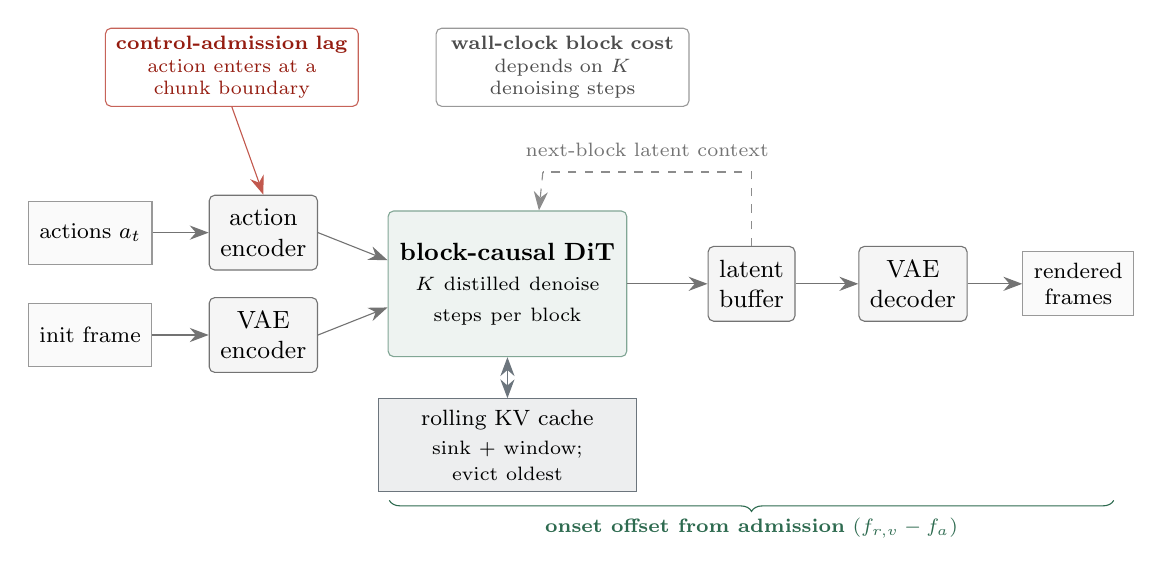
\begin{tikzpicture}[
  mod/.style={draw=black!55, rounded corners=2pt, fill=black!4, align=center, minimum height=0.95cm, inner sep=4pt, font=\small},
  io/.style={draw=black!40, fill=black!2, align=center, minimum height=0.8cm, inner sep=4pt, font=\footnotesize},
  kv/.style={draw=figgray, fill=figgray!12, align=center, minimum height=0.85cm, inner sep=4pt, font=\footnotesize},
  callout/.style={draw, rounded corners=2pt, align=center, text width=3.0cm, minimum height=0.72cm, inner sep=3pt, font=\scriptsize},
  >={Stealth[length=2.4mm]}
]
\node[io] (act) at (0,0.65) {actions $a_t$};
\node[io] (frame) at (0,-0.65) {init frame};
\node[mod] (aenc) at (2.2,0.65) {action\\encoder};
\node[mod] (venc) at (2.2,-0.65) {VAE\\encoder};
\node[mod, minimum height=1.85cm, text width=2.75cm, fill=figgreen!8, draw=figgreen!60] (dit) at (5.3,0) {\textbf{block-causal DiT}\\[3pt]\scriptsize $K$ distilled denoise\\\scriptsize steps per block};
\node[kv, text width=3.0cm] (kvc) at (5.3,-2.05) {rolling KV cache\\[1pt]\scriptsize sink $+$ window; evict oldest};
\node[mod] (buf) at (8.4,0) {latent\\buffer};
\node[mod] (dec) at (10.45,0) {VAE\\decoder};
\node[io] (out) at (12.55,0) {rendered\\frames};
\draw[->,black!55] (act) -- (aenc);
\draw[->,black!55] (frame) -- (venc);
\draw[->,black!55] (aenc.east) -- ([yshift=3mm]dit.west);
\draw[->,black!55] (venc.east) -- ([yshift=-3mm]dit.west);
\draw[<->,figgray] (dit) -- (kvc);
\draw[->,black!55] (dit) -- (buf);
\draw[->,black!55] (buf) -- (dec);
\draw[->,black!55] (dec) -- (out);
\draw[dashed,black!45] (buf.north) -- (8.4,1.42) --
  node[above=2pt,font=\scriptsize,black!55]{next-block latent context}
  (5.75,1.42);
\draw[->,dashed,black!45] (5.75,1.42) -- ([xshift=4mm]dit.north);

\node[callout, draw=figred!70, text=figred!85!black] (admit) at (1.8,2.75)
  {\textbf{control-admission lag}\\action enters at a chunk boundary};
\draw[->,figred!75] (admit.south) -- (aenc.north);
\node[callout, draw=black!40, text=black!70] (cost) at (6.0,2.75)
  {\textbf{wall-clock block cost}\\depends on $K$ denoising steps};

\draw[decorate,decoration={brace,amplitude=4pt,mirror},figgreen] (3.8,-2.75) -- (13.0,-2.75)
  node[midway,below=3pt,font=\scriptsize,figgreen,align=center]{\textbf{onset offset from admission} ($f_{r,v}-f_a$)};
\end{tikzpicture}%
}
\caption{Streaming world-model inference pipeline. Per-frame actions and an initial frame are encoded; a block-causal diffusion transformer denoises one temporal block at a time against a rolling KV cache, and committed latents are decoded to frames. The serving stack owns nominal admission $f_a$; measured decoder support begins at $f_s$; detector onset from support is $f_{r,v}-f_s$. Separately, wall-clock generation cost depends on the $K$ denoising steps. The VAE's four-frame temporal granularity is a representation scale, not a quantity that can be added to $K$.}
\label{fig:pipeline}
\end{figure}

\begin{figure}[t]
\centering
\resizebox{\textwidth}{!}{%
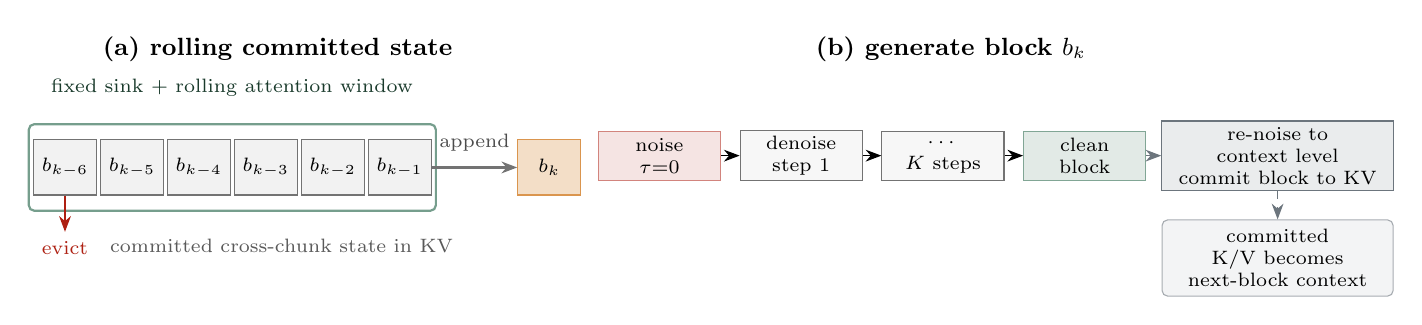
\begin{tikzpicture}[
  blk/.style={draw=black!55, fill=black!5, minimum width=0.8cm, minimum height=0.7cm, inner sep=0, font=\scriptsize},
  cur/.style={blk, fill=figorange!22, draw=figorange!70},
  dstep/.style={draw=black!55, fill=black!3, minimum width=1.55cm, minimum height=0.62cm, inner sep=2pt, font=\scriptsize, align=center},
  >={Stealth[length=2mm]}
]
% left panel: committed rolling state
\node[font=\small\bfseries] at (2.7,1.5) {(a) rolling committed state};
\foreach \i/\j in {0/{k-6},1/{k-5},2/{k-4},3/{k-3},4/{k-2},5/{k-1}}{
  \node[blk] (b\i) at (\i*0.85,0) {$b_{\j}$};
}
\draw[figgreen!65, thick, rounded corners=2pt] (-0.46,-0.55) rectangle (4.71,0.55);
\node[font=\scriptsize, figgreen!55!black, anchor=south] at (2.12,0.78)
  {fixed sink $+$ rolling attention window};
\node[cur] (bk) at (6.15,0) {$b_k$};
\draw[->, thick, black!55] (b5.east) -- (bk.west)
  node[midway,above=2pt,font=\scriptsize,black!70]{append};
\draw[->, figred] (b0.south) -- ++(0,-0.46)
  node[below,font=\scriptsize,figred,align=center]{evict};
\node[font=\scriptsize, align=center, black!65] at (2.75,-1.0)
  {committed cross-chunk state in KV};

% right panel: one-block denoising and commit
\node[font=\small\bfseries] at (11.25,1.5) {(b) generate block $b_k$};
\node[dstep, fill=figred!12, draw=figred!55] (n) at (7.55,0.15) {noise\\$\tau{=}0$};
\node[dstep] (s1) at (9.35,0.15) {denoise\\step $1$};
\node[dstep] (s2) at (11.15,0.15) {$\cdots$\\$K$ steps};
\node[dstep, fill=figgreen!14, draw=figgreen!60] (clean) at (12.95,0.15) {clean\\block};
\node[dstep, fill=figgray!14, draw=figgray, text width=2.8cm, minimum height=0.88cm] (write) at (15.4,0.15)
  {re-noise to context level\\commit block to KV};
\draw[->] (n) -- (s1);
\draw[->] (s1) -- (s2);
\draw[->] (s2) -- (clean);
\draw[->,figgray] (clean) -- (write);
\node[draw=figgray!60, rounded corners=2pt, fill=figgray!8, font=\scriptsize, align=center, text width=2.7cm] (next) at (15.4,-1.15)
  {committed K/V becomes\\next-block context};
\draw[->,figgray,dashed] (write.south) -- (next.north);
\end{tikzpicture}%
}
\caption{Block-causal generation, unrolled. (a) Committed blocks occupy a fixed-size KV window; committing $b_k$ appends its state and evicts the oldest block. (b) One block is produced by $K$ denoising steps, re-noised to the context level, and committed for the next block. Speculation forks at a commit boundary, rollback restores that state, and adaptive compute varies $K$.}
\label{fig:genloop}
\end{figure}

\paragraph{Definition and undetected outcomes.}
Let $f_c$ be the generated-video frame aligned with a user control change, $f_a$ the nominal pixel coordinate of the first latent block whose conditioning includes the changed action, $f_s$ the first raw rendered frame in that latent's measured decoder support when available, and $f_{r,v}$ the detector-defined motion-onset frame in view $v$. The onset is a rendered-frame endpoint of a sustained crossing, not necessarily the earliest perceptually visible effect. We define
\[
\begin{aligned}
\mathrm{\caol}_{\mathrm{frames},v}&=f_{r,v}-f_c,
&\qquad \mathrm{admission\ lag}&=f_a-f_c,\\
\mathrm{decoder\ alignment}&=f_s-f_a,
&\qquad \text{onset from support}_v&=f_{r,v}-f_s.
\end{aligned}
\]
Thus $\mathrm{\caol}_{\mathrm{frames},v}=(f_a-f_c)+(f_s-f_a)+(f_{r,v}-f_s)$. Canonical scoring measures $f_s$ directly and begins the paired search at the flow interval entering that support frame. Each side-by-side raw frame is split into two views, converted to grayscale, and resized to $240\times160$; the signal is the $10\%$ trimmed mean L2 disagreement between aligned dense Farneb\"ack flow fields in the fixed region $x\in[12,228)$, $y\in[20,120)$. Thresholds use only duplicate unchanged-action calibration rollouts, are frozen before intervention scoring, and require a three-sample strict crossing. Wall-clock response is a separate timestamp chain.

\paragraph{Invalidated legacy evidence.}
Earlier offline 48-view action-onset results and magnitude-only plots were generated with an action helper incompatible with the canonical protocol. They are excluded from this manuscript and provide no evidence for any action-result claim. All reported action results below require canonical action-protocol hashes, fresh controls/nulls, raw-support checks, and passed gates.

\section{Mid-stream re-conditioning and control admission}
\label{sec:serving}

\paragraph{Driver.}
The released checkpoints expose only a one-shot API: actions fixed up front, $189$ frames out. Internally, however, generation is block-causal. We expose that structure two ways. The \emph{dispatcher} driver patches the model's conditioning-function constructor to switch between two action streams at a chosen block boundary during a stock rollout. The \emph{session} driver reimplements the block loop as an externally steppable object with per-block action choice, per-block wall-clock timing, per-block denoising schedules, and KV-cache fork/restore. Dispatch keys on the loop's latent-frame index rather than token offsets, whose runtime stride differs from the naive latent-geometry calculation.

\paragraph{Canonical-only evidence policy.}
The earlier four-seed serving pilot used the incompatible helper and is
invalidated. Its tables, figures, onset counts, and lag estimates are removed
rather than retained as descriptive evidence. The driver description above is
implementation context only; quantitative action claims begin with the
canonical matched-control study below.

\section{Matched-control response and incremental timing}
\label{sec:causal}

\paragraph{Confirmatory design.}
We denote the STOP intervention once as forward$\to$stay; its unchanged control is forward$\to$forward. Pair members share the scene, seed, initial image, prompt, checkpoint, and deterministic execution settings. The grid crosses two scenes (\texttt{buildTower\_normal} and \texttt{buildHouse\_flat}), six held-out test seeds, and two admission policies, yielding $24$ scene--seed--policy pairs. A command aligned to $f_c=96$ is admitted at latent index $27$ or $30$, whose nominal pixel coordinates are $108$ and $120$ ($12$ and $24$ frames of control-admission lag). Direct hybrid-latent decoding measures their first raw rendered support at frames $105$ and $117$.

The paired signal is the $10\%$ trimmed mean L2 disagreement between aligned dense Farneb\"ack flow fields inside the fixed region of interest. Thresholds are fitted separately for each scene and view using duplicate unchanged-action rollouts at calibration seeds $101$--$103$, then fixed before intervention scoring. A disjoint null-validation seed ($104$) produces zero strict crossings for all four scene--view thresholds. Deterministic null pairs yield threshold $0$; equality never counts, and an onset requires three consecutive strictly positive samples. Intervention outputs are excluded from threshold fitting. Under these deterministic matched conditions, a crossing identifies divergence attributable to the changed action; it is not a claim of universal causality.

\paragraph{Decoder support and validity.}
A $24$-probe hybrid-latent sweep finds that latent index $t>0$ first affects raw rendered frame $4t-3$. No probe changes an earlier raw pixel, the support is monotone, and repeated decoding is bit-exact. MP4 reconstruction moves apparent differences $39$ frames earlier, so compressed video is diagnostic only and confirmatory scoring uses raw pre-codec frames. Every pair must have exact pre-admission latents, zero raw difference before measured support, finite flow, valid hashes for required artifacts, and matching config, protocol, checkpoint, tokenizer, source commit, and archived source-patch identity.

\paragraph{Confirmatory result.}
All $24/24$ planned scene--seed--policy pairs satisfy the analysis criteria. Treating seed as the statistical unit and scenes/views as repeated observations, both-view and any-view paired detection are $100\%$ for both policies. Mean paired flow-divergence onset lag is $9.0$ frames (seed-bootstrap $95\%$ interval $[9.0,9.0]$) under the $12$-frame admission policy and $21.0$ frames ($[21.0,21.0]$) under the $24$-frame policy. Their paired difference is exactly $12$ frames across all six seeds. Mean continuous peak flow-field divergence is $0.0172288$ and $0.0171567$ detector-grid pixels/frame.

Measured effective full-rollout throughput is $0.834309$ FPS for the shorter policy, with interval $[0.831234,0.837557]$. The longer policy yields $0.835026$ FPS, with interval $[0.831762,0.838335]$. Their relative difference is $0.085889\%$, inside the fixed $5\%$ comparability check. The canonical manifest binds the action-protocol hash, source/config/protocol identities, fresh controls and nulls, and all scored outputs.

\begin{figure}[H]
\centering
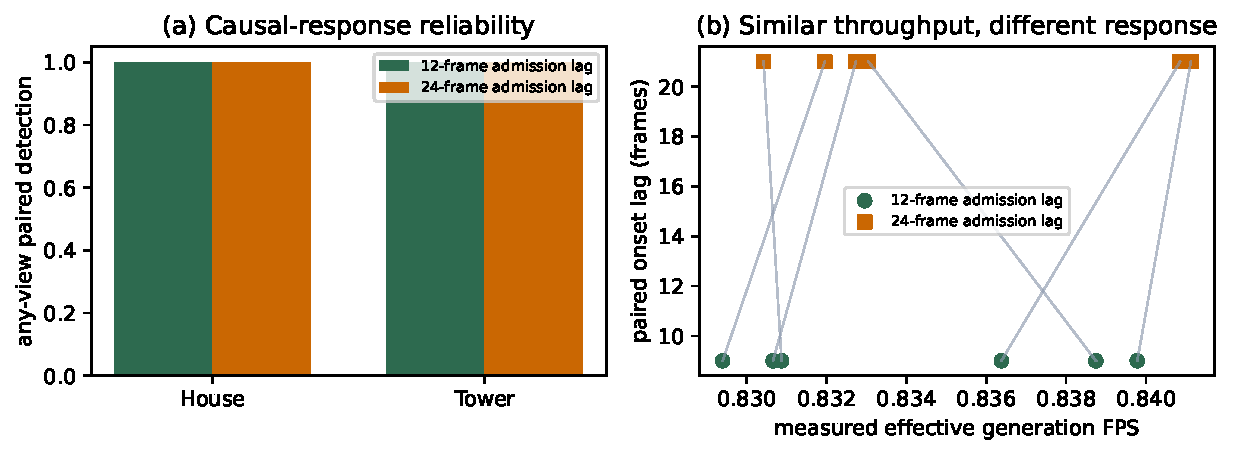
\includegraphics[width=0.95\textwidth]{figures/causal_summary.pdf}
\caption{Matched-control confirmatory results. (a) Every valid pair has a calibrated divergence onset in at least one view in both scenes; both-view detection is also $100\%$. (b) Seed-level scene averages compare measured effective generation throughput with conditional paired onset lag; lines join admission policies for the same seed.}
\label{fig:causal}
\end{figure}

\paragraph{Directional-detector audit.}
Fresh controls, nulls, and \DirectionalInterventions{} intervention rollouts cover forward-to-back and forward-to-true-yaw under the shared action-protocol hash; all $24/24$ interventions are valid. Held-out paired flow-field scoring detects divergence attributable to the changed action for $100\%$ of seeds in both scenes and both transitions. The signed-direction thresholds were fixed before held-out scoring, and the audit fails for back cosine/radial criteria and true-yaw horizontal direction. We therefore report paired divergence only; directional obedience failed and is not inferred from the $100\%$ divergence rate.

\begin{figure}[H]
\centering
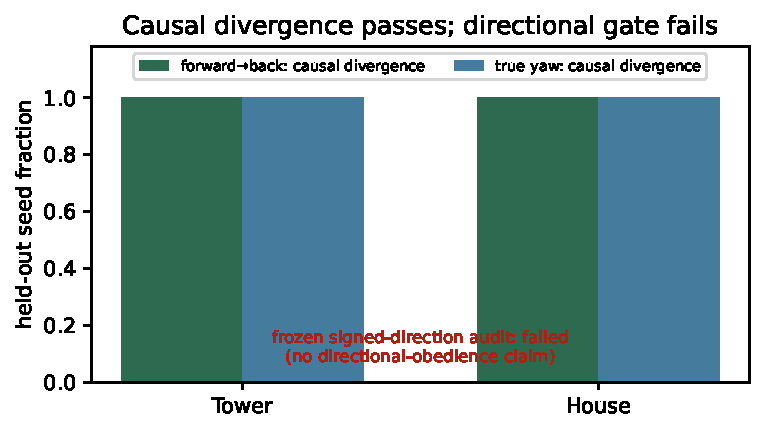
\includegraphics[width=0.62\textwidth]{figures/directional_summary.pdf}
\caption{Directional audit. Paired divergence is detected for back and true yaw in both scenes, while the pre-specified signed-direction criteria fail.}
\label{fig:directional}
\end{figure}

\paragraph{Exact incremental wall-clock chain.}
The steppable session driver records monotonic timestamps for synthetic action receipt, admission, denoising completion, context-cache commit, cached incremental VAE decode, device readiness, synchronous host transfer, and host callback consumption. The benchmark is locked to \texttt{buildTower\_normal}, seeds $301$--$302$, with counterbalanced policy order. Mean action-to-host-ready time is $21{,}476.2\pm29.2$\,ms for the $12$-frame policy and $32{,}930.3\pm958.3$\,ms for the $24$-frame policy, where $\pm$ is descriptive sample SD across $n=2$ seeds. All four runs match full-prefix raw uint8 decoding in both views with maximum error $0$ and zero dropped frames.

\begin{figure}[H]
\centering
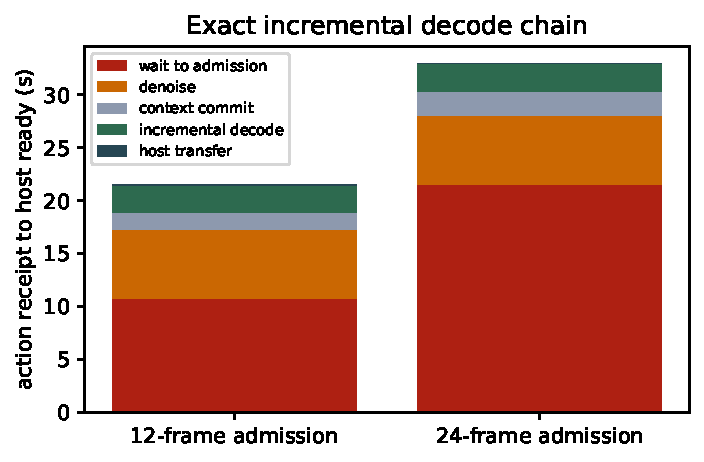
\includegraphics[width=0.58\textwidth]{figures/incremental_wallclock.pdf}
\caption{Canonical incremental wall-clock decomposition. ``Host callback'' is synchronous host consumption, not physical display presentation.}
\label{fig:frame-ready}
\end{figure}

\section{Three inference methods on the session driver}
\label{sec:methods}

All three mechanisms are implemented against the session driver and share the evaluation framework of Section~\ref{sec:bench}. Numbers below are single-scenario measurements on one H200. The paged copy-on-write and deep-copy values are repeated microbenchmarks; the steady-state block reference averages six blocks after discarding two warm-up blocks. Other operation-level fork, restore, rollback, and full-rollout schedule values are one-observation measurements without variability estimates. Figure~\ref{fig:frontiers} collects the measured operating points.

\begin{figure}[H]
\centering
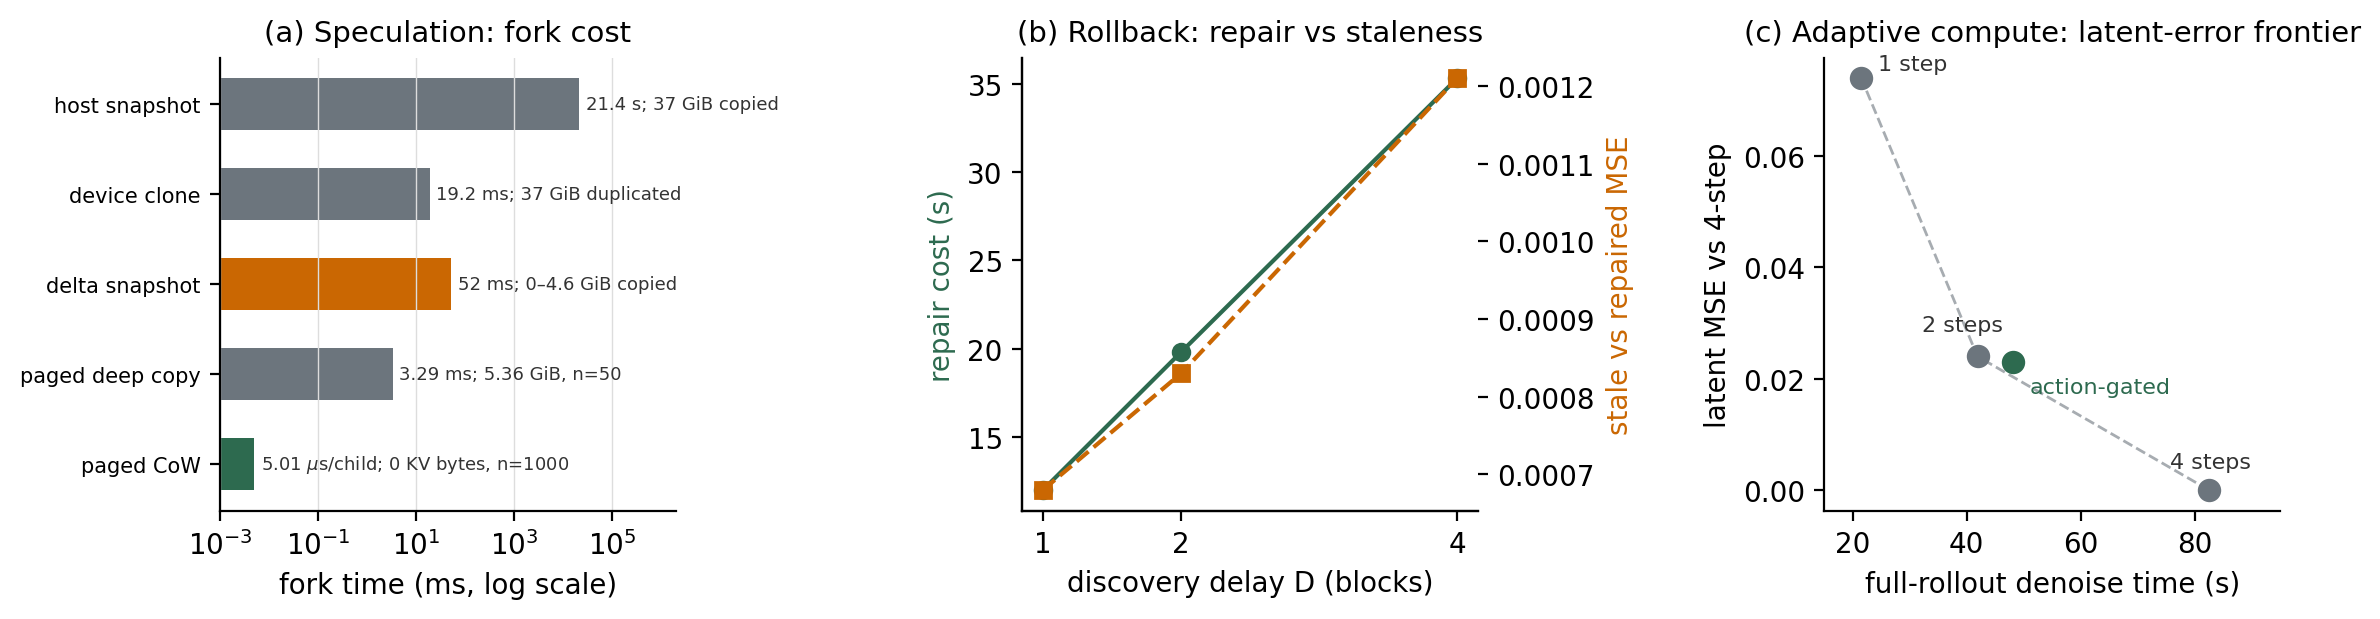
\includegraphics[width=\textwidth]{figures/method_frontiers.png}
\caption{Measured systems operating points. (a) Fork time, log scale, annotated with state duplicated at fork. The paged deep-copy and COW points are the controlled repeated comparison ($n=50$ and $n=1{,}000$); the COW value is per child branch, with four timed calls constructing four-way fan-out. The contiguous-layout points are one-observation values on different paths and resident sizes. The COW operation duplicates block-table/refcount metadata and copies no tensor bytes. (b) One rollback run at each discovery delay, with repair time and stale-versus-repaired latent MSE. (c) One full rollout per denoising schedule, shown as a compute--latent-error frontier; latent MSE is not a perceptual-fidelity metric.}
\label{fig:frontiers}
\end{figure}

\subsection{Speculative action branches}
\label{sec:spec}

At a block boundary, fork the KV cache, pre-generate the next block under $B$ likely action continuations before the user's action arrives, and accept the matching branch or fall back to on-demand generation. Here $B$ is the speculative branch budget; $K$ remains the number of denoising steps per block. On-demand generation costs the block denoise time; accepting a pre-generated branch costs a state swap. Whether speculation wins therefore depends on fork cost, pre-generation budget, and branch hit rate. Table~\ref{tab:fork} and Figure~\ref{fig:frontiers}a give the measured fork landscape.

\paragraph{Trace frontier and exact proposal/refinement.}
The trace corpus contains $597$ episodes of human Minecraft gameplay released with Video PreTraining (VPT)~\cite{vpt}: $512$ train and $85$ held-out test episodes. These are human action logs, not trajectories generated by a streaming world model; we use them only to estimate next-action predictability. Test scoring covers $28{,}310$ eligible episode-local blocks, including $21{,}397$ intent changes. A train-only Markov-1 predictor with $B=4$ hits $59.1381\%$ of intents overall (whole-episode bootstrap $95\%$ interval $[56.7646,61.4038]\%$) and $47.3197\%$ on changes ($[44.4826,50.1101]\%$). Exact 12-frame sequence hashes are much sparser: $9.6044\%$ overall and $2.0984\%$ on changes at $B=4$.

The exact $B=1$ transaction evaluates denoise forward 1 before the action, retains the noisy latent, and restores the parent without context commit; an exact action-hash hit runs forwards 2--4 and commits once, while a miss discards the proposal and generates all four forwards on demand. All \ProposalCheckpointCount{} completed latent/output/live-KV/raw-uint8 checks match their references with maximum error \ProposalMaxError{}. The requested steady-roll eight-block continuation could not run because block 9 plus eight successors needs 51 tokenizer normalization slots while the stock checkpoint has 50.

We call block 0 the \emph{initial block}, block 8 the \emph{first rolling boundary}, where the full attention window first evicts history, and later saturated blocks \emph{steady rolling boundaries}. At the initial block, proposal p50/p95 is \PreRollProposalMedianMs{}/\PreRollProposalTailMs{}\,ms and passes 750\,ms. A known exact hit saves p95 \PreRollCommitSaveTailMs{}\,ms to final commit and \PreRollHostSaveTailMs{}\,ms to synchronous host readiness, with zero errors or drops. This is a wall-clock readiness result at a fixed admission boundary, not a reduction in frame-domain admission lag. The VPT set contains \PreRollEligibleDecisions{}/\VPTEligibleBlocks{} decisions (\PreRollEligibleFraction{}) at later unsaturated indices 1--7, but readiness at those boundaries was not measured. Proposal p95 at the first and steady rolling boundaries is \FirstRollProposalTailMs{}/\SteadyRollProposalTailMs{}\,ms, so the overall readiness criterion fails and $B=2$ is untested. The train-only exact selector covers \ExactConfidenceCoverage{} at \ExactConfidencePrecision{} precision; applying initial-block timing to the later trace decisions projects \ExactConfidenceWorkDeltaMs{}\,ms more proposal-inclusive compute than all-on-demand.

An approximate-intent variant has proposal p95 \IntentProposalTailMs{}\,ms and fails the latent MSE, PSNR, SSIM, and continuation criteria; its pre-specified policy rejects all held-out proposals. It supports no perceptual, semantic, directional, or \caol{} claim. Fused attention is faster but byte-inexact and rejected; compilation and CUDA-graph attempts fail, while cross-attention caching and a preallocated workspace are unsupported. The measured bottleneck is rolling sparse-hub forward compute, not fork or capture. No general profitable speedup is established.

\begin{figure}[H]
\centering
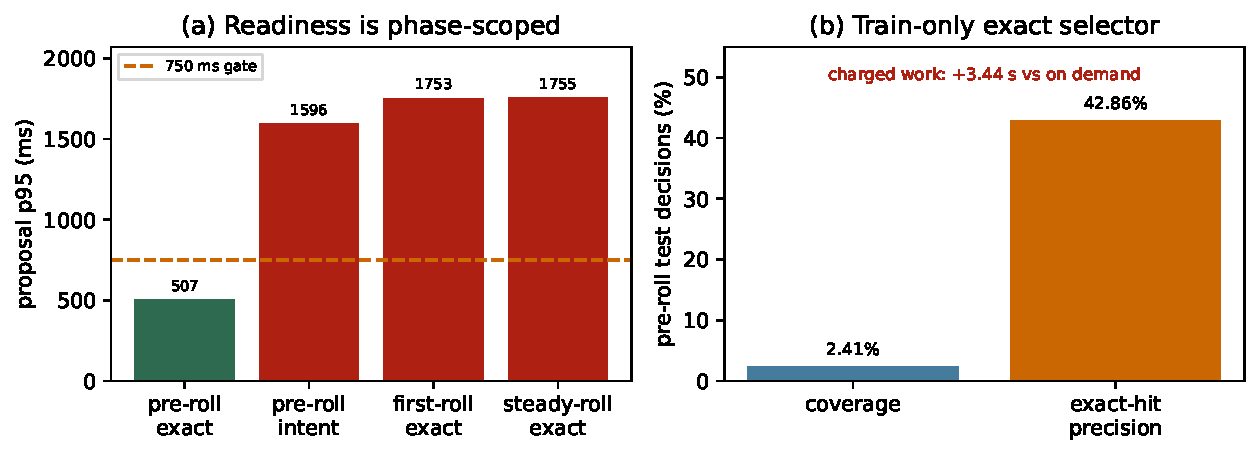
\includegraphics[width=0.9\textwidth]{figures/proposal_refine_summary.pdf}
\caption{Proposal/refinement boundary. The exact initial-block proposal passes the 750-ms readiness criterion, whereas approximate intent and exact rolling-cache proposals fail; the exact selector increases proposal-inclusive compute.}
\label{fig:speculation-frontier}
\end{figure}

The proposal/refinement transaction and contiguous delta path are distinct from the paged copy-on-write microbenchmark below. Paged COW is not substituted into the measured $\gamma$-World transaction and does not establish a profitable end-to-end policy.

\begin{table}[t]
\centering
\caption{Fork cost and incremental state on one H200. Rows 1--3 use $\gamma$-World's contiguous cache; the final row uses the paged AR-diffusion allocator. Detailed protocols and controlled comparisons are given in the text.}
\label{tab:fork}
\small
\begingroup
\renewcommand{\arraystretch}{1.18}
\setlength{\tabcolsep}{5pt}
\begin{tabularx}{\textwidth}{@{}L{3.5cm}C{1.7cm}C{2.7cm}Y@{}}
\toprule
\textbf{Mechanism} & \textbf{Fork} & \textbf{Restore / accept} &
\textbf{Incremental state at fork} \\
\midrule
Full snapshot to host RAM &
$21.4$\,s & $4.2$\,s & $37$\,GiB copied to host \\
\addlinespace[2pt]
Full device clone &
$19.2$\,ms & -- & $37$\,GiB duplicated on GPU \\
\addlinespace[2pt]
Delta snapshot (contiguous) &
$52$\,ms & $85$\,ms / $6.6$\,ms & $0$--$4.6$\,GiB copied on GPU \\
\addlinespace[2pt]
\textbf{Paged copy-on-write}\\\emph{(per child)} &
\textbf{$5.0\,\mu$s} & \textbf{Table swap} &
\textbf{Metadata only; $0$ KV bytes copied} \\
\bottomrule
\end{tabularx}
\endgroup
\end{table}

The contiguous and paged rows use different cache layouts, resident sizes, and software paths and are therefore not a controlled cross-row speedup comparison. The controlled comparison for the paged fork is the repeated deep-copy baseline on the same $5.36$\,GiB resident state.

\paragraph{The contiguous case: exact delta snapshots.}
The $\gamma$-World implementation evaluated here uses a contiguous rolling KV buffer. A full fork of its $37$\,GiB allocated cache is either a host-RAM round trip ($21.4$\,s) or a device clone ($19.2$\,ms with allocation included, but with another $37$\,GiB of GPU residency). Our \emph{delta snapshot} exploits the evaluated implementation's index-derived slice writes and deterministic rolling-window eviction. An exact on-GPU undo stores three end-index scalars per layer plus the prefix destroyed by the roll: zero tensor bytes before the window fills and one $4.6$\,GiB block after it fills. At the first rolling boundary, a one-observation measurement gives $52$\,ms to snapshot and $85$\,ms to restore. Conditional on an already generated matching branch, installing its captured one-block state takes $6.6$\,ms versus a six-block steady-state mean of $4{,}730$\,ms for on-demand block generation. The $6.6$\,ms value excludes proposal generation and does not incorporate branch hit probability. Max-absolute latent difference is $0.0$ against matched runs for the speculated block, restore-then-regenerate path, branch swap, and continuation. The implementation is scoped to one speculated block per branch because deeper branches accumulate multiple rolling shifts.

\paragraph{The paged case: copy-on-write forks.}
A paged KV layout in the style of vLLM~\cite{pagedattention} advances the attention window by dropping block-table entries rather than shifting live cache tensors. As part of this work, we implemented a paged AR-diffusion session fork and proposed it upstream in vLLM-Omni PR~\#4909~\cite{vllmomni}.\footnote{\url{https://github.com/vllm-project/vllm-omni/pull/4909}, draft and open at manuscript preparation; evaluated head commit \texttt{ef77add7}.} On top of the allocator, the fork copies the two classifier-free-guidance block tables and increments physical-page reference counts for committed history. It is a host-side metadata/refcount operation over GPU-resident KV state, not a GPU kernel.

We repeat the session-fork path $1{,}000$ times after $100$ warm-ups while constructing four-way fan-out. Each timed \texttt{ARDiffusionKVState.fork} call creates one child session and forks both CFG streams. CUDA is synchronized before every timer start, although the timed operation itself is host-only. With two $20$-entry CFG block tables and $5.36$\,GiB of GPU tensor state resident but untouched, median fork time is $5.01\,\mu$s per child branch (p10--p90: $4.63$--$5.52\,\mu$s). No tensor bytes are copied at fork time. For comparison, $50$ cold-output-allocation deep copies after $5$ warm-ups have median $3.29$\,ms (p10--p90: $3.27$--$11.17$\,ms); a warm-allocator baseline has median $3.17$\,ms. Both clone timings include allocation of the output tensors and duplicate $5.36$\,GiB. Branches allocate their own future KV pages as they advance.

This result validates the KV-state primitive, not arbitrary full-session replay. Forks are legal only at chunk-commit boundaries; the positive and negative classifier-free-guidance streams must fork atomically; future pages are branch-local; RNG state must also be captured for deterministic replay; and observation-derived conditioning outside the KV pool must be reconstructed for each branch. The current image-conditioning pool permits run-one-branch-at-a-time execution and is not a proof of safe interleaving with arbitrary external session state. \planned{measure concurrent workers and realized arbitrary-action \caol{} without substituting paged-COW timings for the contiguous $\gamma$-World replay.}

\subsection{Rollback-and-re-denoise (barge-in repair)}
\label{sec:rollback}

When an action change is discovered $D$ blocks late (for example under chunked admission or network jitter), stale blocks may already have been generated and displayed. Rollback restores the KV snapshot at the switch block and re-denoises the tail under the new actions. One run at each $D\in\{1,2,4\}$ gives total repair times of $12.0$, $19.8$, and $35.3$\,s on the session driver; regenerated blocks themselves take approximately $6.2$\,s each. Stale-versus-repaired latent MSE is $0.00068$, $0.00083$, and $0.00121$, respectively. These are measured operating points, not a fitted scaling law. \planned{add a splice-continuity metric and repeat the frontier at scale.}

\subsection{Action-gated adaptive compute}
\label{sec:adaptive}

The distilled model spends $4$ denoising steps on every block regardless of control state. In one full rollout per schedule (Table~\ref{tab:adaptive}, Figure~\ref{fig:frontiers}c), using $2$ steps reduces denoising time from $82.5$ to $41.9$\,s with latent MSE $0.024$ relative to the $4$-step output; $1$ step takes $21.5$\,s at MSE $0.074$. An action-gated schedule (four steps for two blocks after the control change and two elsewhere) takes $48.1$\,s with latent MSE $0.023$. This is a compute--latent-error result, not evidence of perceptual equivalence. \planned{separate switch-adjacent from steady-state error and test whether latent MSE tracks perceptual judgments for this four-step-distilled checkpoint.}

\begin{table}[t]
\centering
\caption{Denoising-schedule frontier on the session driver (full $189$-frame rollout, forward$\to$stop scenario). Latent MSE is against the $4$-step reference.}
\label{tab:adaptive}
\begin{tabular}{lrr}
\toprule
schedule & total denoise time & latent MSE vs $4$-step \\
\midrule
$4$ steps (reference) & $82.5$\,s & $0$ \\
$2$ steps & $41.9$\,s & $0.024$ \\
$1$ step & $21.5$\,s & $0.074$ \\
action-gated ($4$ near switch, else $2$) & $48.1$\,s & $0.023$ \\
\bottomrule
\end{tabular}
\end{table}

Absolute times are driver-specific. The earlier ${\sim}0.94$\,s stock-engine observation measured one denoise forward, not a complete block: a candidate requires four denoise forwards plus context commit. The steppable session path runs $4.7$--$6.2$\,s for that complete work. Ratios within a driver are more informative than cross-driver absolute values.

\section{Benchmark Protocol: The Latency--Responsiveness Frontier}
\label{sec:bench}

Section~\ref{sec:causal} instantiates one matched slice of the frontier: two admission policies at nearly equal measured throughput, with paired response reliability, frame-domain onset, decoder support, and host-ready timing. A complete benchmark should additionally vary chunk size, denoising schedule, speculative-branch budget, and rollback depth while reporting measured effective or steady-state FPS, control-admission lag, decoder alignment, paired onset from support, undetected rates, continuous effect magnitude, host-ready time, regeneration or repair rate, KV memory, and long-horizon coherence. Matched unchanged-action controls and separately calibrated thresholds are required before attributing onset to a changed action. A complete benchmark should report frontier curves showing the throughput and systems cost at which changed-action response remains reliable and prompt under matched conditions. \planned{expand the grid across transitions and inference mechanisms and replicate it on a second open-weight streaming model.}

\section{Limitations}
\label{sec:limits}

Paired optical-flow divergence requires visible motion contrast and is not a calibrated perceptual threshold. The STOP result is restricted to two scenes, six test seeds, two admission policies, and one model family. Under deterministic matching, back and true-yaw interventions identify divergence attributable to the changed action, but the pre-specified signed-direction criteria fail, so directional obedience is not supported. Earlier offline and four-seed serving results used an incompatible helper and are excluded.

The incremental timing benchmark uses two seeds per policy and reports descriptive sample SD only. Its host callback is synchronous software consumption, not physical presentation, compositor, or scanout. The proposal/refinement result is $B=1$ on one H200: its positive gate is restricted to pre-saturation block 0, rolling gates fail, $B=2$ is untested, and neither exact-confidence nor approximate-intent selection establishes aggregate benefit. It measures systems exactness/readiness/work, not arbitrary-action \caol{} or perceptual equivalence; paged COW is a separate controlled allocator result. Annotation and QC infrastructure exists for 48 canonical primary intervention views and 16 QC items, but no annotators have participated; human validation remains pending. The paged copy-on-write result validates KV bookkeeping and write isolation, while deterministic complete-session replay still requires RNG and non-KV state capture. Second-model replication remains future work.

\section{Conclusion}
\label{sec:conclusion}

Frame rate alone is an incomplete contract for interactive world models, because a stream can run at nearly unchanged throughput while control response shifts by a full block. Control-aligned onset latency separates serving-owned admission, measured decoder alignment, and detector onset from raw support. Under deterministic matched conditions, unchanged-action controls distinguish divergence attributable to the changed action from ordinary world dynamics.

In the two-scene STOP study, all $24$ planned scene--seed--policy pairs are valid and both views detect paired divergence for every seed. Increasing admission lag from $12$ to $24$ frames shifts mean paired flow-divergence onset from $9$ to $21$ frames while effective generation throughput changes by only $0.085889\%$. Exact incremental timing reaches host readiness in $21.476$ versus $32.930$\,s without claiming physical presentation. Exact proposal/refinement passes the 750-ms criterion only at the initial block. The trace contains $582$ decisions at later unsaturated indices, but their readiness was not measured; rolling and selection criteria fail, so no general profitable speedup is established. The exact transaction, the initial-block result, and the rolling sparse-hub bottleneck delimit what the current system can support. The paged session fork remains a separate allocator result.

\paragraph{Reproducibility: environment.}
The $\gamma$-World source commit is \texttt{6a95de85}. The local instrumentation patch has SHA-256 prefix \texttt{814691ca7fbb} and is archived with the experiment summaries. The checkpoint repository is \path{chijw/Gamma-World}; the file is \path{causal-few-step/model.safetensors}, from Hugging Face snapshot \texttt{8e15162f3e49}. Inference uses one process and one NVIDIA H200 reporting $143{,}771$\,MiB HBM, driver 580.159.04, CUDA toolkit/runtime 13.0, Python 3.10.20, PyTorch 2.9.0+\texttt{cu130}, cuDNN 9.13, OpenCV 5.0.0, NumPy 2.2.6, and pandas 2.3.3. Model weights and KV tensors are bfloat16; action tensors, initial video preprocessing, latent noise, and session output buffers are float32. The canonical action protocol has SHA-256 \texttt{90e8c77467e1361f0}\allowbreak\texttt{4b99740097c5fd96}\allowbreak\texttt{aab8b0d3ae6a9b90}\allowbreak\texttt{2879de0a5983e15}. Calibration uses seeds $101$--$103$, null validation uses $104$, causal testing uses $201$--$206$, and incremental timing uses $301$--$302$. The repeated paged-fork microbenchmark uses the same H200 and CUDA~13.0 with Python~3.12.3, PyTorch~2.11.0+\texttt{cu130}, vLLM~0.22.0, and vLLM-Omni PR head \texttt{ef77add7}.

\paragraph{Reproducibility: state and timing.}
The rollout has $16$ blocks of $3$ latent frames, a $24$-latent-frame (eight-block) attention window, and $3{,}600$ spatial tokens per latent frame per view. At the first rolling block, summing \texttt{numel}$\times$\texttt{element\_size} over allocated KV tensors gives $37{,}842$\,MiB; one destroyed rolling prefix is $4{,}730.2$\,MiB. Canonical rollouts require hashed latent, raw uint8 decode, and resized detector-frame artifacts. The $24$ hybrid decoder probes cover latent indices $24$--$47$ and compare raw pre-MP4 pixels. Seed-bootstrap intervals use $20{,}000$ deterministic resamples after averaging scenes within each seed; views are never treated as independent seeds. Incremental timing uses \texttt{perf\_counter\_ns}, synchronizes CUDA at GPU boundaries, validates every increment against full-prefix raw uint8 decoding, and transfers ready frames synchronously to host. The steady-state block reference for method measurements is the arithmetic mean of six blocks after discarding the first two; other contiguous-cache fork/restore values are single observations, rollback uses one run at each depth, and adaptive compute uses one $16$-block rollout per schedule.

The repeated paged benchmark times the actual \texttt{ARDiffusionKVState.fork} host path over two $20$-entry CFG block tables while $5.36$\,GiB in $30$ GPU tensors remains resident and untouched. Each timed call creates one child session, including both CFG streams; four such calls construct the measured four-way fan-out. The protocol uses $100$ warm-ups and $1{,}000$ measured per-child forks, with CUDA synchronization immediately before every start. The comparison uses $5$ warm-ups and $50$ measurements for each deep-copy condition, synchronizing before and after each copy. The cold condition clears cached output storage before the timer, forcing \texttt{clone} to allocate its $5.36$\,GiB output inside the timed region; the warm condition reuses allocator storage. Raw samples and percentile summaries are provided as the arXiv ancillary file \texttt{anc/data/cow\_microbench.json}. Hash-bound confirmatory gates, per-view and per-pair scores, bootstrap summaries, decoder-support results, directional-audit outputs, timestamp event logs, and the exact source patch are retained in the v2 reproducibility bundle. The streaming driver, measurement scripts, v2 reproducibility bundle, paper source, and ancillary data are public at \url{https://github.com/arun-elr/caol-streaming-world-models}. The paged fork and tests are public in vLLM-Omni PR~\#4909.

\begin{thebibliography}{99}
\bibitem{causvid} T.~Yin, Q.~Zhang, R.~Zhang, et~al. From slow bidirectional to fast autoregressive video diffusion models. \emph{CVPR}, 2025. \emph{arXiv:2412.07772}.
\bibitem{selfforcing} X.~Huang, Z.~Li, G.~He, M.~Zhou, and E.~Shechtman. Self forcing: Bridging the train-test gap in autoregressive video diffusion. \emph{NeurIPS}, 2025. \emph{arXiv:2506.08009}.
\bibitem{causalrcm} K.~Zheng, G.~He, M.~Zhao, J.~Zhang, H.~Chen, J.~Chen, C.-H.~Lin, M.-Y.~Liu, J.~Zhu, and Q.~Ma. Causal-rCM: A unified teacher-forcing and self-forcing open recipe for autoregressive diffusion distillation in streaming video generation and interactive world models. \emph{arXiv:2606.25473}, 2026.
\bibitem{motionstream} J.~Shin, Z.~Li, R.~Zhang, et~al. MotionStream: Real-time video generation with interactive motion controls. \emph{ICLR}, 2026. \emph{arXiv:2511.01266}.
\bibitem{vllmomni} P.~Yin, J.~Zhu, H.~Gao, et~al. vLLM-Omni: Fully disaggregated serving for any-to-any multimodal models. \emph{arXiv:2602.02204}, 2026.
\bibitem{vpt} B.~Baker, I.~Akkaya, P.~Zhokhov, et~al. Video PreTraining (VPT): Learning to act by watching unlabeled online videos. \emph{NeurIPS}, 2022. \url{https://github.com/openai/Video-Pre-Training}.
\bibitem{specdecode} Y.~Leviathan, M.~Kalman, and Y.~Matias. Fast inference from transformers via speculative decoding. \emph{ICML}, PMLR 202:19274--19286, 2023.
\bibitem{pagedattention} W.~Kwon, Z.~Li, S.~Zhuang, et~al. Efficient memory management for large language model serving with PagedAttention. \emph{SOSP}, pp.~611--626, 2023. \url{https://doi.org/10.1145/3600006.3613165}.
\bibitem{mira} A.~Hu, V.~Volhejn, A.~Ramanana Rahary, et~al. Multiplayer interactive world models with representation autoencoders. \emph{arXiv:2607.05352}, 2026. \url{https://mira-wm.com}.
\bibitem{gammaworld} F.~Liu, K.~He, T.~Shen, et~al. Gamma-World: Generative multi-agent world modeling beyond two players. \emph{arXiv:2605.28816}, 2026.
\bibitem{dreamzero} S.~Ye, Y.~Ge, K.~Zheng, et~al. World action models are zero-shot policies. \emph{arXiv:2602.15922}, 2026.
\bibitem{cosmos3} NVIDIA et~al. Cosmos 3: Omnimodal world models for physical AI. \emph{arXiv:2606.02800}, 2026.
\bibitem{oasis} Decart, J.~Quevedo, Q.~McIntyre, S.~Campbell, X.~Chen, and R.~Wachen. Oasis: A universe in a transformer. Project report, 2024. \url{https://oasis-model.github.io/}.
\bibitem{gamengen} D.~Valevski, Y.~Leviathan, M.~Arar, and S.~Fruchter. Diffusion models are real-time game engines. \emph{ICLR}, 2025. \emph{arXiv:2408.14837}.
\bibitem{mineworld} J.~Guo, Y.~Ye, T.~He, et~al. MineWorld: A real-time and open-source interactive world model on Minecraft. \emph{arXiv:2504.08388}, 2025.
\bibitem{wan} Team Wan, Ang~Wang, Baole~Ai, et~al. Wan: Open and advanced large-scale video generative models. \emph{arXiv:2503.20314}, 2025.
\bibitem{ltx} Y.~HaCohen, N.~Chiprut, B.~Brazowski, et~al. LTX-Video: Realtime video latent diffusion. \emph{arXiv:2501.00103}, 2024.
\bibitem{hunyuanvideo} W.~Kong, Q.~Tian, Z.~Zhang, et~al. HunyuanVideo: A systematic framework for large video generative models. \emph{arXiv:2412.03603}, 2024.
\end{thebibliography}

\end{document}
